\documentclass[12point]{article}

\usepackage{amsmath,amsthm,amsfonts,amssymb,mathdots}

\usepackage{hyperref}

\linespread{.9}

\hoffset=-.25in
\voffset=-.7in
\oddsidemargin=0in
\evensidemargin=0in
\topmargin=0in
\textwidth=7.1in
\textheight=9.6in

\def\i{{\mathbf{i}}}
\def\j{{\mathbf{j}}}
\def\k{{\mathbf{k}}}
\def\u{{\mathbf{u}}}
\def\v{{\mathbf{v}}}
\def\w{{\mathbf{w}}}
\def\m{{\mathbf{m}}}
\def\a{{\mathbf{a}}}
%\def\b{{\mathbf{b}}}
\def\p{{\mathbf{p}}}
\def\q{{\mathbf{q}}}
\def\r{{\mathbf{r}}}
\def\T{{\mathbf{T}}}
\def\N{{\mathbf{N}}}
\def\B{{\mathbf{B}}}
\def\A{{\mathbf{A}}}

\def\row{{\mathbf{row}}}
\def\ker{{\mathbf{ker}}}
\def\Im{{\mathbf{Im}}}



\def\Z{{\mathbb Z}}
\def\R{{\mathbb R}}
\def\F{{\mathbb F}}
\def\C{{\mathbb C}}

\def\End{{\bf End}}
\def\rmspan{{\bf span}}



\def\e{\vec{\bf e}}
\def\f{\vec{\bf f}}
\def\0{\vec{\bf 0}}

\def\d{{\bf d}}
\def\b{{\bf b}}
\def\c{{\bf c}}
\def\r{{\bf r}}
\def\x{{\bf x}}
\def\y{{\bf y}}
\def\z{{\bf z}}
\def\rref{{  \buildrel{\rm row\ ops} \over \longrightarrow  }}
\def\proj{{\rm proj}}


\def\fiverm{}
\input pictex.tex
\input prepictex.tex
\input postpictex.tex


\def\F{{\mathbf{F}}}


\def\R{{\mathbb{R}}}

\usepackage{graphicx}

\begin{document}

\pagestyle{headings}
\thispagestyle{empty}

\begin{centering}
{\large \sffamily MATH/COMP-365 Computational Linear Algebra}
\hfill
{\large \sffamily Name $\underline{\hskip2.5truein}$}\\
{\large \sffamily {Spring 2020}}
\hfill
{\large \sffamily  $\phantom{x}$}\\
\bigskip\bigskip %\bigskip\bigskip
\hfill
\centerline{\Large \sffamily \bfseries{Midterm 1}}
\hfill\break
\bigskip
\centerline{\large\sffamily Due Tuesday, March 10,  2020 (in class and R Markdown file submitted to Moodle before class)}
\end{centering}
\noindent \textsf{
\begin{itemize}
\item The exam is open notes, open Moodle, open R, and open book.  You may not use the internet, except in the case of looking up coding help (and the caveat in problem 6).
\item \textbf{It is not okay to talk to each other or anyone else about the exam! This of course includes discussing how you solve problems, but it even includes things like asking, ``how is it going?" or ``which problem are you working on?" or making comments like ``problem 5 is easy." }
\item Please show and explain all of your work so that I can give you as much partial credit as possible. However, do not turn in information that is not germane to your solution.
\item You are welcome to use any of the R functions in 365Functions.r
\item The first 5 problems would constitute the `in-class' portion of the exam and the last 3 would be the `take-home'.
\item The first 6 problems may be hand-written on this answer sheet. If you'd like to LaTeX them up, I've included the exam file for you to do so, but this is not required.
\item The last two problems should be submitted as a knitted html or pdf document coming from an R Markdown file that contains your code, relevant calculation output, plots, as well as your written explanations. Make sure that this file is readable and clear. You should use the R Markdown template provided. If you use R on any of the other problems, add them to this file, but make sure to have problems and answers clearly labeled. \textbf{You must submit this file in Moodle as well as make a print-out as discussed below.}
\item All of these documents (your handwritten answer sheet and your html R Markdown document) should be printed out and stapled together to be turned in on the due date. 
\item Hints: I may give a small hint or a little help with R for free.  If you are really stuck, I may sell a hint for points so that you can move forward. I will warn you of the point value before I sell you anything.  
\item I may reserve some ``style'' points for the clarity of your work and the quality of your computation. That is, I may possibly take some points off if you get the right answer,  but do it in a confusing or clumsy or inefficient way. (It is still true, though, that it's okay to use a loop even if vectorization is possible).
\end{itemize}}
\bigskip

$$
\begin{tabular}{|c|c|c| }
\hline
Problem  & Point Value & Your Score \\ \hline
1&7& $\vphantom{\Big|}$ \\ \hline
2&10& $\vphantom{\Big|}$ \\ \hline
3&10& $\vphantom{\Big|}$ \\ \hline
4&15& $\vphantom{\Big|}$ \\ \hline
5&16& $\vphantom{\Big|}$ \\ \hline
6&12& $\vphantom{\Big|}$ \\ \hline
\textcircled{7}&15& $\vphantom{\Big|}$ \\ \hline
\textcircled{8}&15& $\vphantom{\Big|}$ \\ \hline
Total     & 100 & $\vphantom{\Big|}$ \\  \hline
\end{tabular}
$$
\bigskip

\noindent{\sffamily Please sign the following (if you are able) and be sure to turn in this cover sheet with your exam:}

{\sl
I pledge my honor that I have not participated in any dishonest
work on this exam, nor do I know of dishonest work done by other
students on this exam.}

\bigskip\bigskip
\centerline{\underbar{$\phantom{Lori Ziegelmeier and Mike Neuberg and Quinlyn and Zoe}$}}
\centerline{(signature)}
\bigskip

%\noindent{\sffamily As an alternative to signing this page, you may also type out this pledge as part of your submission.}
\addtocounter{page}{-1}



\newpage
\begin{enumerate}
%%%%%%%%%%%%%%%%%%%%%%%%%%%%%%%%%%%%%%%%%%%%%%%%%%
% Question 1

\item (7 points)
For all parts of this problem, I am using the same computer and software. I have a $1000 \times 1000$ symmetric positive definite matrix $A$. On this machine, I solve $A\x=\b$ for a particular choice of $\b$ in 10 seconds, as efficiently as possible using a direct method discussed in class.

\begin{enumerate}
\item (4 points) I would also like to solve a second problem $B\y=\c$ on the same machine, where $B$ is a dense $100000 \times 100000$ matrix without any particularly nice structure and $\c$ is a $100000 \times 1$ vector. Approximately how many hours will it take to solve $B\y=\c$?
\vspace{2.75in}

\item (3 points) I have a third matrix $C$ that is a $1000 \times 1000$ dense matrix without any particularly nice structure, and I would like to solve $C\z=\d$ for one hundred different values of $\d$. How long should I expect it to take to solve the 100 problems
$$ C\z=\d_1,~~~~C\z=\d_2,~~~~C\z=\d_3,~~\ldots~~,~~~~C\z=\d_{100} $$
with the same $C$ matrix and 100 different $\d$ vectors, as efficiently as possible? (Just circle one answer. No justification is necessary.)
\medskip

\begin{itemize}
\item[(i)] Approximately 10 seconds
\item[(ii)] Approximately 100 seconds
\item[(iii)] Approximately 1,000 seconds
\item[(iv)] Approximately 10,000 seconds
\item[(v)] Approximately 100,000 seconds
\item[(vi)] Approximately 1,000,000,000,000 seconds
\end{itemize}  
\bigskip
\vspace{.7in}
\end{enumerate}


%%%%%%%%%%%%%%%%%%%%%%%%%%%%%%%%%%%%%%%%%%%%%%%%%%
% Question 2


\newpage
\item (10 points)
Before the iPhone, there was the hPhone. Unfortunately, the hPhone had a serious design flaw. While the rest of the world was designing 32-bit and 64-bit phones, the hPhone was {\bf a 16-bit machine that used one bit for the sign, 8 bits for the mantissa, and 7 bits for the exponent}:
\medskip

$$
\begin{tabular}{|c|cccccccc|ccccccc|}
\hline
$\pm$ & m&a& n & t  &  i & s &s &a&   && e & x & p &&  \\
\hline
$\cdot$&
$\cdot$&$\cdot$&$\cdot$&$\cdot$&$\cdot$&$\cdot$&$\cdot$&$\cdot\phantom{\Big| x}$ 
&$\cdot$&$\cdot$&$\cdot$&$\cdot$&$\cdot$&$\cdot$&$\cdot$ \\
\hline
\end{tabular}
$$
\bigskip

\begin{enumerate}

\item (3 points) An exponent bias of 63 is used in this system, so 63 is subtracted from the stored value to get the actual exponent, or 63 is added to the actual exponent before it is stored. We are then able to store exponent values from -62 to +63 (saving -63 and +64 for subnormal numbers and INF, respectively). 
\medskip

Which number below is the best approximation of the largest (finite) exactly representable number on the hPhone? (Just circle one answer. No justification is necessary.) 

\medskip

\begin{itemize}
\item[(i)] $10^6$
\item[(ii)] $10^{10}$
\item[(iii)] $10^{19}$
\item[(iv)] $10^{31}$
\item[(v)] $10^{63}$
\item[(vi)] $10^{307}$
\end{itemize}

\bigskip

\item (4 points) The decimal number -45.4375 converts to binary as -101101.0111.  How will this number be stored in your machine? Make sure to show how you calculated your answer.

$$
\begin{tabular}{|c|cccccccc|ccccccc|}
\hline
$\pm$ & m&a& n & t  &  i & s &s &a&   && e & x & p &&  \\
\hline
\phantom{\Big| x}&
\phantom{\Big| x}&\phantom{\Big| x}&\phantom{\Big| x}&\phantom{\Big| x}&\phantom{\Big| x}&\phantom{\Big| x}&\phantom{\Big| x}&\phantom{\Big| x}
&\phantom{\Big| x}&\phantom{\Big| x}&\phantom{\Big| x}&\phantom{\Big| x}&\phantom{\Big| x}&\phantom{\Big| x}& \phantom{\Big| x}\\
\hline
\end{tabular}
$$

\vspace{2in}


\item (3 points)
On the hPhone, the difference between $2^8$ and the smallest number larger than $2^8$ that is exactly representable is: (Just circle one answer. No justification is necessary.)
\medskip

\begin{itemize}
\item[(i)] less than the difference between 1 and the smallest number larger than 1 that is exactly representable
\item[(ii)] the same as the difference between 1 and the smallest number larger than 1 that is exactly representable
\item[(iii)] greater than the difference between 1 and the smallest number larger than 1 that is exactly representable
\end{itemize}
\end{enumerate}  


\newpage




%%%%%%%%%%%%%%%%%%%%%%%%%%%%%%%%%%%%%%%%%%%%%%%%%%
% Question 3


\newpage

\item (10 points) One of the classical laws of planetary motion due to Kepler says that a planet revolves around the sun in an elliptic orbit obeying $M=E-e\sin(E)$. Here, $M$ is a parameter called the mean anomaly and $e$ is the eccentricity of the Earth. These are known quantities. You can use Kepler's law to solve for $E$, which is called the eccentric anomaly.

In the code block below, I've solved for $E$ using a root-finding algorithm you are (likely) not familiar with. The sequence of approximations is stored in the variable $E$, and you can consider the last element of that vector to be the exact answer.

\begin{verbatim}
M <- 1
e <- 0.0167
f <- function(E){M+e*sin(E)-E}
fp <- function(E){e*cos(E)-1}
fpp <- function(E){-e*sin(E)}
rs <- function(E){E - f(E)/fp(E)-(f(E)/fp(E))^2*fpp(E)/2/fp(E)}
steps <- 6
E <- 201.5
for (i in 1:steps){
  E[i+1] <- rs(E[i])
}
E

#This is the output of E
201.500000 -151.111170   66.192872    9.401840    1.125484    1.014177    1.014179 
\end{verbatim}

\begin{enumerate}
	\item (6 points) How fast does this root finding algorithm converge on this specific problem? Explain your answer. You may use R, but you are not required to do so. If you do, make sure to include your code.
	\begin{itemize}
\item[(i)] Slower than linearly
\item[(ii)] Linearly
\item[(iii)] Faster than linearly but slower than quadratically
\item[(iiii)] Quadratically
\item[(iiiii)] Faster than quadratically
\end{itemize}
\vfill

\item (4 points) How does this compare to the order of convergence for Newton's method on this problem? How about the bisection method? Explain your answers. 
\vspace{.05in}

\emph{Hint: You should NOT have to do any computations to answer this part (b).} 
\vfill
 
\end{enumerate}



\newpage

%%%%%%%%%%%%%%%%%%%%%%%%%%%%%%%%%%%%%%%%%%%%%%%%%%
% Question 4

\item (15 points) Let $A=\begin{bmatrix} 1 & -1 & -1 & -1 & \ldots & -1 \\ 0 & 1 & -1 & -1 & \ldots & -1 \\ 0 & 0 & 1 & -1 & \ldots & -1 \\ \vdots & \vdots & \vdots & \vdots & \vdots & \vdots \\ 0 & 0 & 0 & 0 & 0 & 1 \end{bmatrix}$.
\begin{enumerate}
	\item (5 points) Show that $||A||_2 \geq \sqrt{n}$. Hint: For this problem and the next you might find the standard basis vector $\e_n=\begin{bmatrix} 0 \\ \vdots \\ 0 \\ 1 \end{bmatrix} $ useful.
	\vfill
	\item (5 points) Give a lower bound for $\kappa_2(A)$ (the matrix condition number in the 2-norm). 
	\vfill
	\item (3 points) Would you say that the $n \times n$ matrix $A$ is a well-conditioned matrix (for large n)? \\
	\textbf{Yes or No (Circle one)}. Briefly justify your answer below.
	\vspace{1in}
	
	\item (2 points) How does your previous answer relate to the error in computing $A\x=\b$? 
	\vspace{0.5in}
\end{enumerate}


\newpage

%%%%%%%%%%%%%%%%%%%%%%%%%%%%%%%%%%%%%%%%%%%%%%%%%%
% Question 5


\item (16 points) There are many different ways to rank and rate teams and individuals in competitions. The following is the method behind one of the computer rankings that previously was used to determine the college football playoff teams.

For each team $i$, the computer knows the following information:
\begin{itemize}
\item $w_i=$ the number of wins for team $i$
\item $l_i=$ the number of losses for team $i$
\item $t_i=w_i+l_i=$ the total number of games played by team $i$
\end{itemize}
The goal is to determine $\r$, a vector of ratings, with the $i^{th}$ element $r_i$ representing the rating for team $i$. Rankings are just the order of the ratings (the highest $r_i$ is given the \#1 ranking spot, etc.).

The ratings are computed as follows:
\begin{align} \label{Eq:colley}
r_i = \frac{1}{2+t_i}\left(1+\frac{w_i-l_i}{2}+\sum\limits_{j \in \{i\hbox{'s opponents}\}}r_j\right).
\end{align}
where opponent means a team that a particular team played (not all the other teams in the league).
\footnote{
Note 1: If team $i$ played team $j$ multiple times (say $k$ times), then $r_j$ is counted $k$ times in the summation on the right-hand side of \eqref{Eq:colley}. This summation term is an adjustment for strength of schedule.
}
\footnote{
Note 2: For this ranking system, the margin of victory does not matter, and exactly who you beat does not matter, except through the effect of your opponents' ratings on your strength of schedule.}

\begin{enumerate}
\item (8 points) Try out this rating system on some partial data from the 2019 football scedule. Here are the results of 10 matches between 5 teams -- Augsburg (A), Carleton (C), Hamline (H), St. Olaf (O), and St. Thomas (T):


\begin{center}
\begin{tabular}{ccccc}
O beat C& T beat H &O beat A & O beat H& C beat H\\
T beat A& C beat A & T beat C& T beat O& A beat H\\
\end{tabular}
\end{center}

When combined for every team $i$, equation $\eqref{Eq:colley}$ represents a system of $n$ (6 in this case) equations with $n$ unknowns (the ratings). For our small example, convert this system of equations into the form $A\r=\b$, and then use R's \texttt{solve} function to find the ratings vector $\r$. Make a small table with the team names and their ratings, ordered from highest to lowest.
\bigskip
\vspace{1in}

$A=$
\vspace{1.5in}

$\b=$\hspace{1in}$\r=$\hspace{1.2in} $\begin{tabular}{|c|c|c| }
\hline
Rank & College & Rating \\ \hline
1&\phantom{Gustavus Adolphus}& $\phantom{\Big|}$ \\ \hline
2&\vphantom{\Big|}& \phantom{Gustavus Adolphus} \\ \hline
3&\vphantom{\Big|}& $\vphantom{\Big|}$ \\ \hline
4&\vphantom{\Big|}& $\vphantom{\Big|}$ \\ \hline
5&\vphantom{\Big|}& $\vphantom{\Big|}$ \\ \hline
\end{tabular}$

\vspace{1in}

\newpage
%\item (3 points) For this ranking method, the matrix $A$ is always symmetric positive definite (we can prove it together next week). What is the best direct method to solve $Ar=b$? \emph{Briefly} justify your answer.
%\vspace{2.5in}

\item (4 points) Let's say that we are using this ranking system to rank hundreds of thousands to millions of chess players around the world (let's say $n$ players), where each player has played on the order of 100 games.\footnote{We'll assume that the network is connected (i.e., if you choose any random players $i$ and $j$, you can find a sequence of other players $k_1, k_2,\ldots,k_M$ such that $i$ played $k_1$, who played $k_2$, and so forth until $k_M$, who played $j$).} Which of the following best describes the computational complexity of a single iteration of the Jacobi method to solve $Ar=b$? Note that I've left out constants that do not depend on $n$.  Circle one and \emph{briefly} justify your answer.
\begin{itemize}
\item[(i)] ${\cal O}(n)$
\item[(ii)] ${\cal O}(n^2)$
\item[(iii)] ${\cal O}(n^3)$
\item[(iv)] ${\cal O}(n \log n)$
\end{itemize}
\vspace{1.5in}

\item (4 points) For the chess ranking application, which of the following statements is true? Circle one and \emph{briefly} justify your answer. 
\begin{itemize}
\item[(i)] Jacobi's method will never converge.
\item[(ii)] Jacobi's method will always converge.
\item[(iii)] Jacobi's method may or may not converge. It will depend on the data of how many games each person played, who beat whom, etc.
\end{itemize}
\bigskip
\vspace{1.5in}

\end{enumerate}


\newpage

%%%%%%%%%%%%%%%%%%%%%%%%%%%%%%%%%%%%%%%%%%%%%%%%%%
% Question 6

\item (12 points) In this problem, you will learn about a sparse matrix storage format. Use an internet search engine to find what is available/popular, and choose one to write about. We will consider the following $6 \times 6$ sparse matrix throughout this problem.
$$A=\begin{bmatrix} \cdot & 7 & \cdot & \cdot & 2 & \cdot \\ -1 & \cdot & \cdot & \cdot & \cdot & 5 \\ \cdot & \cdot & \cdot & 3 & \cdot & \cdot \\ \cdot & 4 & \cdot & \cdot & 2 & \cdot \\ \cdot & \cdot & 9 & \cdot & \cdot & \cdot \end{bmatrix}$$
\begin{enumerate}
	\item (4 points) Use this matrix to illustrate one of the commonly adopted storage formats for sparse matrices, making sure to explain how you are storing the nonzero entries.
	\vfill
	\item (4 points) List one main advantage and one main disadvantage of the format you choose.
	\vfill
	\item (4 points) Write a pseudocode for matrix-vector multiplication using this format. Then, illustrate this with $A\x$ where $\x=\begin{bmatrix} 2 \\ 3 \\ 5 \\ 1  \\4 \\ 6 \end{bmatrix}$.
	\vfill
\end{enumerate}



\newpage
%%%%%%%%%%%%%%%%%%%%%%%%%%%%%%%%%%%%%%%%%%%%%%%%%%
% Question 7


\item (15 points) In this problem, we are going to use sparse matrices to represent chemical graphs of organic molecules, and then use eigenvalues to analyze where two molecules might bridge (connect).\footnote{This is an idea discussed in a paper here: https://arxiv.org/abs/1611.06959. You are welcome to read this article, but you do not have to look at it at all in order to do this problem. Full disclosure: I have not run this application by a chemist. So while the math and computing are sure to be interesting, the interpretations may not be chemically accurate due to my desire to simplify the problem and use tools we know.} 


\begin{figure}[h]
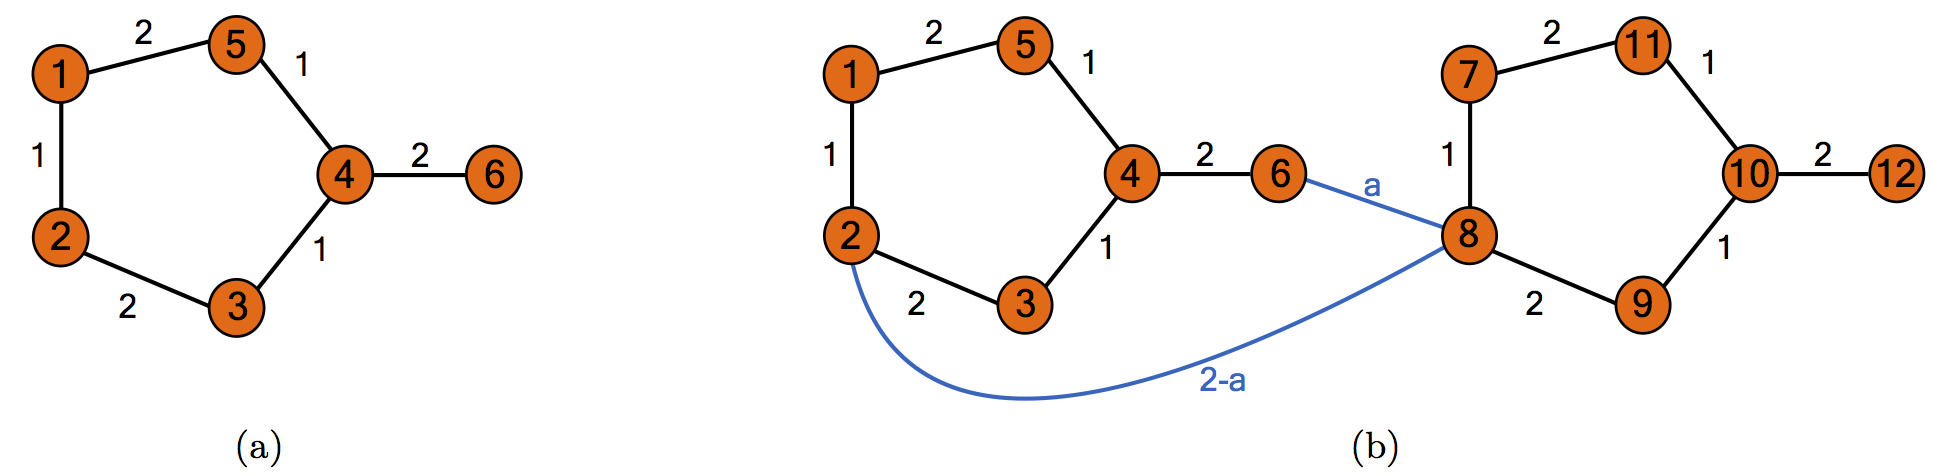
\includegraphics[width=.98\linewidth]{fig1} 
\caption{(a) Voltage graph for a single fulvene molecule. (b) Two fulvene molecules connected with two extra edges.}
\end{figure}

Figure 1(a) shows the voltage graph for a single fulvene molecule. %, where the edges represent {\color{red} insert}. 
The graphs for two individual molecules can be bridged by adding one or more edges  connecting a vertex from each graph. As an example, in Figure 1(b), we consider adding two new edges (shown in blue), each connecting vertices from each of the initial graphs. The resulting weighted, undirected graph in Figure 1(b) features 12 vertices, labeled 1 through 12. The edges of the graph connecting vertices on the same organic molecule retain their initial edge weights. The two new connecting edges have weights of $a$ (connecting vertices 6 and 8) and $2-a$ (connecting vertices 2 and 8), where $a$ is some number between 0 and 2. The weighted adjacency matrix $W$ for this bridged graph is a $12 \times 12$ matrix, with the $(i,j)^{th}$ entry $W_{ij}$ equal to 0 if there is no edge connecting vertices $i$ and $j$, and equal to the weight of the edge connecting vertices $i$ and $j$ otherwise.

\begin{enumerate}
\item (2 points) Let $a=1$. Create the sparse matrix $W$. Run the command \texttt{image(W)} to make sure your $W$ has the correct sparsity (nonzero) pattern.
\medskip

\item (1 point) The graph Laplacian matrix is defined as $L=D-W$, where $W$ is the weighted adjacency matrix, and $D$ is a diagonal matrix, with the $i^{th}$ diagonal element equal to the degree of vertex $i$; that is, the sum of the weights of the edges leading into vertex $i$. You can compute $D$ with the command \texttt{D=diag(rowSums(W))}. Still using $a=\frac{1}{2}$, form the matrix $L$ and print out its eigenvalues. There should be one zero eigenvalue and the rest should be positive.\footnote{For an undirected graph, the number of graph Laplacian eigenvalues equal to zero is equal to the number of connected components in the graph.} 
\medskip

\item (6 points) The weighted adjacency matrix $W$ has both negative and positive eigenvalues. The spectral gap of $W$ is the difference between the negative eigenvalue closest to 0 and the positive eigenvalue closest to 0. For example, when $a=1$, the negative eigenvalue closest to 0 is -0.755, and the positive eigenvalue closest to 0 is 1.344. So the spectral gap is 2.099.\footnote{According to the paper at https://arxiv.org/abs/1611.06959, this gap represents the difference between the energy of the lowest unoccupied molecular orbital and the energy of the highest occupied molecular orbital. A larger gap implies higher kinetic stability.}
\medskip

We are going to let $a$ vary, and see how it affects the spectral gap. Create a function \texttt{sg(a)} that takes as input a choice of $a$ between 0 and 2, and returns the spectral gap of the graph shown above in Figure 1(b), for the given value of $a$. Plot the function \texttt{sg($\cdot)$} on the interval $[0,2]$.
\medskip

\item (6 points) Now we want to determine for which value of $a$ the spectral gap of the graph shown in Figure 1(b) is maximized. First, use the finite difference derivative function $D$ from Technical Report 1 (you can use yours or mine, which is called \texttt{FDDeriv}) to generate a function $g$ that is the numerical derivative of the \texttt{sg($\cdot$)} function. Plot the function $g(\cdot)$ on the interval $[0,2]$. Then use your favorite root-finding method to find the value of $a$ on the interval $[0,2]$ that maximizes the spectral gap of $W$. For your answer to this question, include a single code block with all of your code. On the last line, execute the command \begin{verbatim}paste("Root =",as.character(root))\end{verbatim} where root is a variable containing your approximation of the root.

\end{enumerate} 

\newpage
%%%%%%%%%%%%%%%%%%%%%%%%%%%%%%%%%%%%%%%%%%%%%%%%%%
% Question 8

\item (15 points) Brownian motion is a simple, continuous, stochastic process that is widely used in physics and finance for modeling random behavior that evolves over time. Quantitative Finance uses a version called ``Geometric Brownian Motion" (GBM) to predict pricing options. The general model we use to determine the future behavior of an asset is: $S_t = S_0 e^{(\mu - \frac{\sigma ^2}{2}) t + \sigma W_t}$, where $S_t$ is the price at time $t$, $S_0$ is the initial price, $\mu$ is the expected return, and $\sigma$ is the standard deviation of the return.

The R implementation of the solution is shown below (no changes need to be made to this code, but look it over carefully to see what it does.):

\begin{verbatim}
GBM <- function(N, sigma, mu, S0, Wt = NULL) {
  # Creates a single asset path of daily prices using Geometric Brownian Motion. 
  # One year is 252 days since that is about how many trading days are in any
  # given year.
  #
  # Inputs:
  #   N: Number of days in the path.
  #   sigma: Standard deviation of daily continuously compounded 
  #          returns (known as volatility).
  #   mu: Average daily continuously compounded returns (known as drift). 
  #   S0: The initial price of the asset. 
  #   Wt: The cumulative Brownian motion of the model. This can be supplied or 
  #       left as NULL. In the case that it is NULL, a vector will be provided.
  #       If you include this argument, it must be a vector of length N of the 
  #       cumulative sum of a random variable to work properly. (Steps i.-iii. below    
  #       create this.) 
  #
  # Returns:
  #   A vector of length N containing the asset prices generated by the specified
  #   GBM. 
  if (is.null(Wt)) {
    Wt <- cumsum(rnorm(N, 0, 1))
  }
  t <- (1:N)/252
  p1 <- (mu - 0.5*(sigma*sigma)) * t
  p2 <- sigma * Wt
  St = S0 * exp(p1 + p2)
  return(St)
}
\end{verbatim}

\begin{enumerate}
	\item (6 points) We are going to simulate the prices of several correlated assets over time, using Correlated GBM. Imagine we have assets that are dependent on each other. Our goal is to predict future asset values taking into consideration correlation of past asset values. The simulation process starts with an $n \times n$ correlation matrix $C$, which shows the correlation between $n$ stocks. The following is the procedure for generating correlated random variables:

\begin{enumerate}
	\item[i.] Perform Cholesky Decomposition on correlation matrix $C$ to obtain upper triangular matrix $R$.
	\item[ii.] Generate a random matrix $X$ with $n$ columns following a standard normal distribution with mean = 0 and variance = 1.
	\item[iii.] Obtain a correlated random matrix $W_t = XR$. This generates a matrix that encodes both randomness and correlation within the problem.
	\item[iv.] Use the above \texttt{GBM} function to generate the daily price path for each asset.
\end{enumerate}

Implement the algorithm described above. Below is a starter of the function:
	
	\begin{verbatim}
	CorrelatedGBM <- function(N, S0, mu, sigma, cor.mat) {
  # Creates a matrix of correlated daily price paths using Geometric 
  # Brownian Motion. 
  #
  # Inputs: 
  #   N: Number of days in the path.
  #   mu: A vector of drift or average daily continuously compounded returns.  
  #   sigma: A vector of volatility or standard deviation of daily continuously   compounded returns. 
  #   S0: A vector of initial prices of the assets. 
  #   cor.mat: The correlation matrix of the daily continuously compounded 
  #            returns. 
  #
  # Returns:
  #   A matrix of simulated daily price paths of length N having the same number
  #   of assets as in the mu and sigma vectors. Note that mu and sigma must have
  #   the same dimensions. 
  
  GBMs <- matrix(nrow = N, ncol = length(mu)) # Generate empty GBM vector for return
  
  # Fill in code below for Step i.
	
  # Step ii. (done for you):
  X <- matrix(rnorm(N * length(mu), 0, 1), ncol = length(mu)) # Generate the Nxn random matrix
  X <- apply(X, 2, cumsum) # cumulate value from random matrix to reflect compounded return.
  
  # Fill in code below for Step iii.
  
  # Fill in code below for Step iv. and store it in GBMs:
  
  return(GBMs)
}
\end{verbatim}

\item (6 points) Delta, United, and American Airlines are the three biggest airlines in the U.S. airline market. The dataset \texttt{AirlineStockPrices.csv} records the stock price for these three stocks starting from July 1, 2007. In order to simulate the stock prices, we need to determine the inputs for the function \texttt{CorrelatedGBM}. Here are the steps you can follow to generate every piece of information you'll need:

\begin{enumerate}
	\item Generate a return matrix by calculating the daily log return. For example, $r_{i,j} = log(\frac{S_{i+1,j}}{S_{i,j}})$ where $r_{i,j}$ denotes the return while $S_{i,j}$ denotes the price for stock $j$ in the $i^{th}$ day.\footnote{If you are curious to know why this works, check out this \href{https://quantivity.wordpress.com/2011/02/21/why-log-returns/}{link}.}
	\item Use the \texttt{cor()} function to calculate the correlation matrix $cor.mat$ on the return matrix.
	\item Calculate the column mean of the return matrix to create the vector of average returns $mu$. 
	\item Calculate the standard deviation of each column of the return matrix to create the vector of standard deviations $sigma$. (HINT: \texttt{sd()} is a function that computes standard deviation. You may find the function \texttt{apply()} useful, but it is not required to use it).
	\item Generate the vector that represents the current price value $S_0$ (that is, the last price available).
\end{enumerate}

\item (1 point) We would like to simulate the price of these stocks over 3 years (remember there are only 252 trading days in a year). Use the \texttt{CorrelatedGBM} function to construct the three paths of these stock prices. Plot the path of these stocks over 3 years using the code below:

\begin{verbatim}
# make correlated asset paths
set.seed(123) # include this so everyone has the same random initialization
paths <- CorrelatedGBM(N, S0 , mu, sigma, cor.mat)

# make a basic r plot 
colors <- c('darkblue', 'darkgreen', 'darkgoldenrod')
t <- (1:N)/252
plot(t, paths[,1], type = 'l', ylim = c(0, max(paths)), xlab = "Year", 
     ylab = "Price", main = "Simulated Asset Prices", col = colors[1])

for (i in 2:ncol(paths)) {
  lines(t, paths[, i], col = colors[i])
}
legend(x = 0.5, y = 145,c('DAL','UAL','AAL'), lty = c(1,1,1), col = colors, cex = 0.7)
\end{verbatim}


\item (2 points) What do you observe about the stock prices? How will you invest based on the simulation?

\end{enumerate}



%\newpage 
%{\bf This is an extra page in case you need more space. Please make sure to label the problem on which you are working.} 
%\newpage
%{\bf This is an extra page in case you need more space. Please make sure to label the problem on which you are working.} 
%\newpage 
%{\bf This is an extra page in case you need more space. Please make sure to label the problem on which you are working.} 
%\newpage
%{\bf This is an extra page in case you need more space. Please make sure to label the problem on which you are working.} 



\end{enumerate}
\end{document}


